%  !TeX  root  =  user_guide.tex

\section{Преобразователь слоев OGR}

% when the revision of a section has been finalized,
% comment out the following line:
%\updatedisclaimer

Преобразователь слоёв OGR дает возможность ковертировать векторные слои
в формат, поддерживаемый библиотекой OGR. \footnotetext{Поддерживаемые
форматы могут варьироваться в зависимости от установленного пакета
GDAL/OGR.} Модуль очень прост в использовании и требует лишь несколько
параметров для выполнения:

\begin{itemize}[label=--]
\item \textbf{Исходный Формат/Набор данных/Слой}: Здесь вводится
формат, поддерживаемый OGR, и путь к конвертируемому векторному файлу.
\item \textbf{Выходной Формат/Набор данных/Слой}: Здесь вводится
формат, поддерживаемый OGR, и путь к результирующему векторому файлу.
\end{itemize}

\begin{figure}[ht]
 \centering
   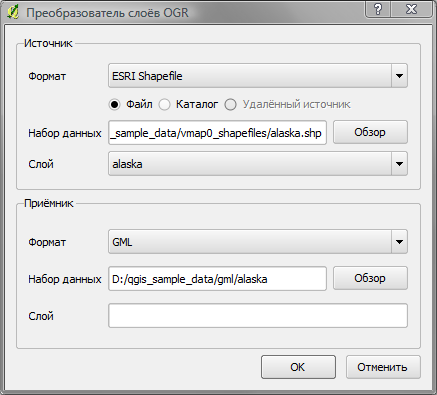
\includegraphics[clip=true, width=7.5cm]{ogr_converter_dialog}
   \caption{Преобразователь слоев OGR \wincaption}\label{fig:ogr_converter_dialog}
\end{figure}

\minisec{Использование модуля}

\begin{enumerate}
  \item Запустить QGIS, загрузить Преобразователь слоёв OGR через
  <<Управление модулями>> (см. Раздел~\ref{sec:load_core_plugin}) и
  нажать на иконку \toolbtntwo{ogr_converter}{Преобразователь слоёв OGR},
  которая появилась на панели инструментов QGIS. На экране появится окно
  <<Преобразователь слоёв OGR>>, как показано на рисунке~\ref{fig:ogr_converter_dialog}.
  \item Выбрать формат, поддерживаемый библиотекой OGR (к примеру,
  \selectstring{ESRI Shapefile}{\ldots}), и путь к исходному
  векторному файлу (например, \filename{alaska.shp}) в блоке <<Источник>>.
  \item Выбрать формат, поддерживаемый библиотекой OGR (к примеру,
  \selectstring{GML}{\ldots}), и прописать путь и название выходного
  векторного файла (к примеру, \filename{alaska.gml}) в блоке <<Приёмник>>.
  \item Нажать \button{Ok}.
\end{enumerate}

\FloatBarrier
